\section{Results}

Results have been corrected for dead pixels, measured dark current, and measured background. Grating is fixed at 300, and pumping wavelength is 800nm. Counts is a number given from the spectrometer which relate to the relative intensity detected by the pixel in the CCD. The excitation laser intensity is the intensity hitting the sample. This intensity is measured before the objective, and calculated using the objective data sheet. Defect dot is a description used about the black dots in the microscope pictures, which can be related to dislocations, etch pits, or other defects in the crystal.

\subsection{R6-Q3-210}

This is the electronic grade sample, with a very low amount of impurities.

\begin{figure}[H]
\centering
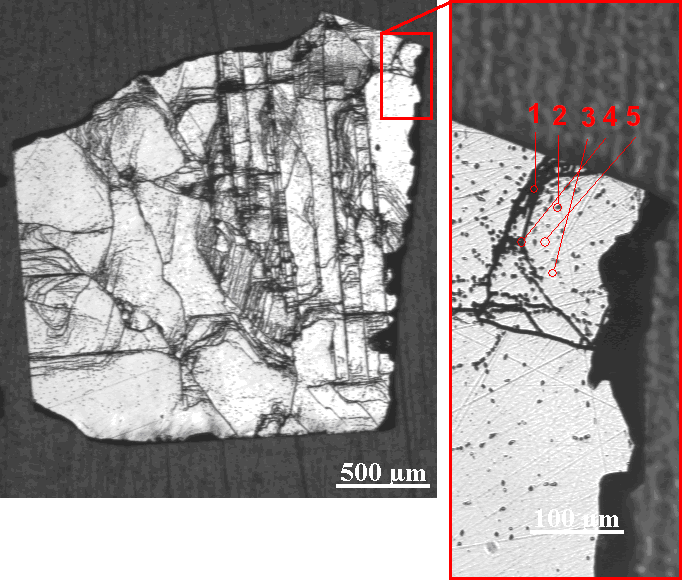
\includegraphics[width=0.7\columnwidth]{R6-Q3-210-A_enlarged}
\caption[R6-Q3-210 A from light microscope]{Sample R6-Q3-210 A picture taken using light microscope. Marked areas are spots where photoluminescence has been measured.}
\label{fig:R6-Q3-210-A_enlarged}%
\end{figure}


\begin{figure}[H]
\centering
\includegraphics[width=0.7\columnwidth]{R6-Area1_dislocation_line-20s}
\caption[R6-Q3-210 at a dislocation line]{Sample R6-Q3-210 A pumped with 128~mW at 10~K in a dislocation line (Area 1 in figure \ref{fig:R6-Q3-210-A_enlarged}).}
\label{fig:R6-Area1_dislocation_line-20s}%
\end{figure}


\begin{figure}[H]
\centering
\includegraphics[width=0.7\columnwidth]{R6-Area2_dislocation_dot-20s}
\caption[R6-Q3-210 at a defect dot]{Sample R6-Q3-210 A pumped with 128~mW at 10~K in a defect dot (Area 2 in figure \ref{fig:R6-Q3-210-A_enlarged}).}
\label{fig:R6-Area2_dislocation_dot-20s}%
\end{figure}


\begin{figure}[H]
\centering
\includegraphics[width=0.7\columnwidth]{R6-Area3_clean_area-20s}
\caption[R6-Q3-210 at a defect free area]{Sample R6-Q3-210 A pumped with 128~mW at 10~K in a defect free area (Area 3 in figure \ref{fig:R6-Q3-210-A_enlarged}).}
\label{fig:R6-Area3_clean_area-20s}%
\end{figure}


\begin{figure}[H]
\centering
\includegraphics[width=0.7\columnwidth]{R6-A-Area4-intensities-grain_boundary-30s}
\caption[R6-Q3-210 at a grain boundary]{Sample R6-Q3-210 A pumped with different intensities at 22~K in a grain boundary (Area 4 in figure \ref{fig:R6-Q3-210-A_enlarged}). Results are Savitzky-Golay filtered for easier comparison.}
\label{fig:R6-A-Area4-intensities-grain_boundary-30s}%
\end{figure}


\begin{figure}[H]
\centering
\includegraphics[width=0.7\columnwidth]{R6-A-Area5-intensities-clean_area-30s}
\caption[R6-Q3-210 at a defect free area]{Sample R6-Q3-210 A pumped with different intensities at 22~K in a defect free area (Area 5 in figure \ref{fig:R6-Q3-210-A_enlarged}). Results are Savitzky-Golay filtered for easier comparison.}
\label{fig:R6-A-Area5-intensities-clean_area-30s}%
\end{figure}








\subsection{ES1-Q3-201}

This sample is from a dirty feedstock, with a large amount of P and B.


\begin{figure}[H]
\centering
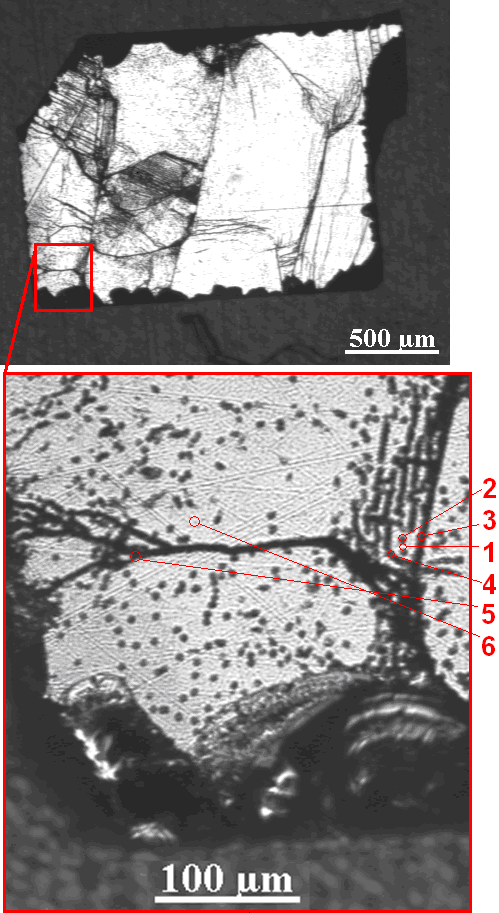
\includegraphics[width=0.85\columnwidth]{ES1-Q3-201-C_enlarged}
\caption[ES1-Q3-201 C from light microscope]{Sample ES1-Q3-201 C 210 A picture taken using light microscope. Marked areas are spots where photoluminescence has been measured.}
\label{fig:ES1-Q3-201-C_enlarged}%
\end{figure}

\subsubsection{Room temperature}

\begin{figure}[H]
\centering
\includegraphics[width=0.7\columnwidth]{ES1-room_temperature}
\caption[ES1-Q3-201 at room temperature]{Sample ES1-Q3-201 A pumped with 20~mW at 295~K in a dislocation line (black) and in a defect free area (blue). An estimated mean dark current offset has been subtracted.}
\label{fig:ES1-room_temperature}%
\end{figure}


\subsubsection{Low temperature}

\begin{figure}[H]
\centering
\includegraphics[width=0.7\columnwidth]{ES1-Area1_dislocation_free-10s}
\caption[ES1-Q3-201 at a defect free area]{Sample ES1-Q3-201 C pumped with 128~mW at 12~K in a defect free area (Area 1 in figure \ref{fig:ES1-Q3-201-C_enlarged}).}
\label{fig:ES1-Area1_dislocation_free-10s}%
\end{figure}

\begin{figure}[H]
\centering
\includegraphics[width=0.7\columnwidth]{ES1-Area2_dislocation_spot-10s}
\caption[ES1-Q3-201 at a defect free area]{Sample ES1-Q3-201 C pumped with 128~mW at 12~K in a defect dot (Area 2 in figure \ref{fig:ES1-Q3-201-C_enlarged}).}
\label{fig:ES1-Area2_dislocation_spot-10s}%
\end{figure}


\begin{figure}[H]
\centering
\includegraphics[width=0.7\columnwidth]{ES1-Area3_grain_boundary_60s}
\caption[ES1-Q3-201 at a grain boundary]{Sample ES1-Q3-201 C pumped with 128~mW at 12~K in a grain boundary (Area 3 in figure \ref{fig:ES1-Q3-201-C_enlarged}). For 60~s integration time, the main TO line at 1.1~eV is saturating the camera.}
\label{fig:ES1-Area3_grain_boundary_60s}%
\end{figure}

\begin{figure}[H]
\centering
\includegraphics[width=0.7\columnwidth]{ES1-Area4_dislocation_line-60s}
\caption[ES1-Q3-201 at a dislocation line]{Sample ES1-Q3-201 C pumped with 128~mW at 14~K in a dislocation line (Area 4 in figure \ref{fig:ES1-Q3-201-C_enlarged}). For 60s integration, the main TO line around 1.1eV is saturating the camera.}
\label{fig:ES1-Area4_dislocation_line-60s}%
\end{figure}



\begin{figure}[H]
\centering
\includegraphics[width=0.7\columnwidth]{ES1-C-Area5-intensities-clean_area-30s}
\caption[ES1-Q3-201 at a defect free area]{Sample ES1-Q3-201 C pumped with different intensities at 22~K in a defect free area (Area 5 in figure \ref{fig:ES1-Q3-201-C_enlarged}). Results are Savitzky-Golay filtered for easier comparison.}
\label{fig:ES1-C-Area5-intensities-clean_area-30s}%
\end{figure}

\begin{figure}[H]
\centering
\includegraphics[width=0.7\columnwidth]{ES1-C-Area6-intensities-grain_boundary-30s}
\caption[ES1-Q3-201 at a grain boundary]{Sample ES1-Q3-201 C pumped with different intensities at 22~K in a grain boundary (Area 6 in figure \ref{fig:ES1-Q3-201-C_enlarged}). Results are Savitzky-Golay filtered for easier comparison.}
\label{fig:ES1-C-Area6-intensities-grain_boundary-30s}%
\end{figure}





\subsection{MH2-Q3-210}

This sample is the same as ES1-Q3-201, except for added chromium in this sample.



\begin{figure}[H]
\centering
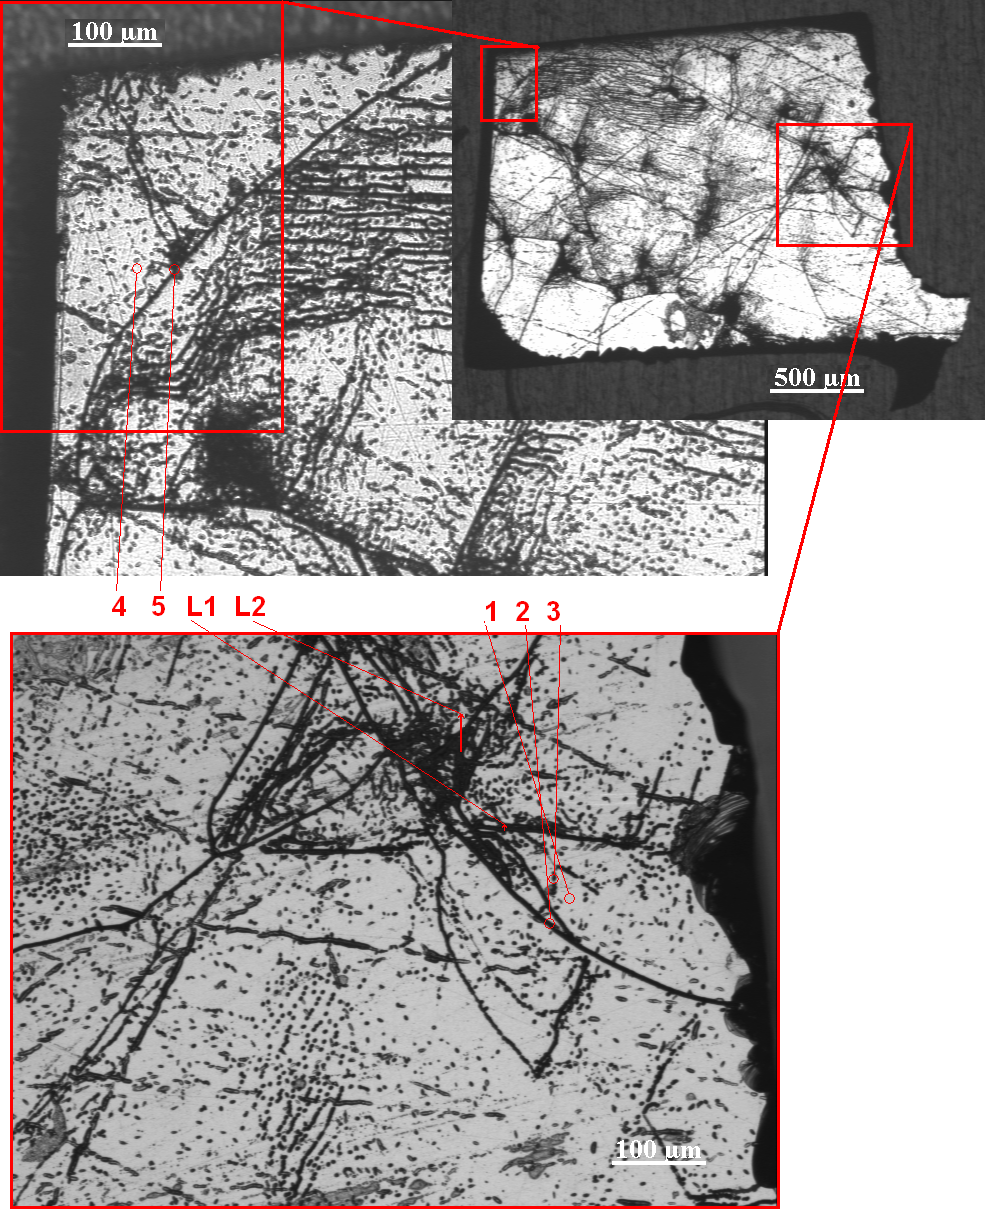
\includegraphics[width=0.85\columnwidth]{MH2-Q3-210-B2_enlarged}
\caption[MH2-Q3-210 B2 from light microscope]{Sample MH2-Q3-210 B2 picture taken using light microscope. Marked areas are spots where photoluminescence has been measured.}
\label{fig:MH2-Q3-210-B2_enlarged}%
\end{figure}



\subsubsection{Room temperature}

\begin{figure}[H]
\centering
\includegraphics[width=0.7\columnwidth]{MH2-room_temperature}
\caption[MH2-Q3-210 at room temperature]{Sample MH2-Q3-210 C pumped with 20~mW at 295~K in a defect free area (blue), and in an area with dislocations (black). An estimated mean dark current offset has been subtracted, and results are Savitzky-Golay filtered for easier comparison.}
\label{fig:MH2-room_temperature}%
\end{figure}

\subsubsection{At 70~K}
%%%TODO double check that it is in fact 20s integration, and not 10s due to low signal / noise floor
\begin{figure}[H]
\centering
\includegraphics[width=0.7\columnwidth]{MH2-70K}
\caption[MH2-Q3-210 at 70K]{Sample MH2-Q3-210 D pumped with 128~mW at 70~K in a defect free area (blue, area 1 in figure \ref{fig:MH2-Q3-210-B2_enlarged}), and in an area with dislocations (black, area 2 in figure \ref{fig:MH2-Q3-210-B2_enlarged})). An estimated mean dark current offset has been subtracted, and results are Savitzky-Golay filtered for easier comparison.}
\label{fig:MH2-70K}%
\end{figure}

\subsubsection{Low temperature}

\begin{figure}[H]
\centering
\includegraphics[width=0.7\columnwidth]{MH2-Area1-dislocation_free-20s}
\caption[MH2-Q3-210 at area 1]{Sample MH2-Q3-210 B2 pumped with 128~mW at 12~K in a defect free area (Area 1 in figure \ref{fig:MH2-Q3-210-B2_enlarged}).}
\label{fig:MH2-Area1-dislocation_free-20s}%
\end{figure}

\begin{figure}[H]
\centering
\includegraphics[width=0.7\columnwidth]{MH2-Area2-dislocation_line-20s}
\caption[MH2-Q3-210 at area 2]{Sample MH2-Q3-210 B2 pumped with 128~mW at 12~K in a dislocation line (Area 2 in figure \ref{fig:MH2-Q3-210-B2_enlarged}).}
\label{fig:MH2-Area2-dislocation_line-20s}%
\end{figure}

\begin{figure}[H]
\centering
\includegraphics[width=0.7\columnwidth]{MH2-Area3-dislocation_dot-60s}
\caption[MH2-Q3-210 at area 3]{Sample MH2-Q3-210 B2 pumped with 128~mW at 12~K in a defect dot (Area 3 in figure \ref{fig:MH2-Q3-210-B2_enlarged}) with 20s integration time (black) and 60s integration time (blue). The 60s integration time has an estimated mean dark current offset subtracted, in addition to measured dark current due to a change in the dark current in between measurements.}
\label{fig:MH2-Area3-dislocation_dot-60s}%
\end{figure}


\begin{figure}[H]
\centering
\includegraphics[width=0.7\columnwidth]{MH2-B2-Area4-intensities-grain_boundary-30s}
\caption[MH2-Q3-210 at area 4 with different intensities]{Sample MH2-Q3-210 B2 pumped with different intensities at 27~K in a grain boundary (Area 4 in figure \ref{fig:MH2-Q3-210-B2_enlarged}). Results are Savitzky-Golay filtered for easier comparison.}
\label{fig:MH2-B2-Area4-intensities-grain_boundary-30s}%
\end{figure}


\begin{figure}[H]
\centering
\includegraphics[width=0.7\columnwidth]{MH2-B2-Area5-intensities-clean_area-30s}
\caption[MH2-Q3-210 at area 5 with different intensities]{Sample MH2-Q3-210 B2 pumped with different intensities at 27~K in a defect free area (Area 5 in figure \ref{fig:MH2-Q3-210-B2_enlarged}). Results are Savitzky-Golay filtered for easier comparison.}
\label{fig:MH2-B2-Area5-intensities-clean_area-30s}%
\end{figure}


\begin{figure}[H]
\centering
\includegraphics[width=0.7\columnwidth]{MH2-B2-Area5-tempereatures-clean_area-30s}
\caption[MH2-Q3-210 at area 5 with different temperatures]{Sample MH2-Q3-210 B2 pumped with 16~mW at different temperatures in a defect free area (Area 5 in figure \ref{fig:MH2-Q3-210-B2_enlarged}). Results are Savitzky-Golay filtered for easier comparison.}
\label{fig:MH2-B2-Area5-tempereatures-clean_area-30s}%
\end{figure}



\subsubsection{Line mapping}

These results are a line mapping of different spots on the sample.

Positions 1-10 has en equally large distance in between them, in a straight line displayed as L1 in figure \ref{fig:MH2-Q3-210-B2_enlarged}.


\begin{figure}[H]
\centering
\includegraphics[width=0.7\columnwidth]{MH2-mapping-small_steps-20s}
\caption[MH2-Q3-210 line mapping]{Sample MH2-Q3-210 B2 pumped with 128~mW at 14~K line map using 10 small steps, on line L1 in figure \ref{fig:MH2-Q3-210-B2_enlarged}.}
\label{fig:MH2-mapping-small_steps-20s}%
\end{figure}



Positions 1-20 has en equally large distance in between them, in a straight line displayed as L2 in figure \ref{fig:MH2-Q3-210-B2_enlarged}.


\begin{figure}[H]
\centering
\includegraphics[width=0.7\columnwidth]{MH2-mapping-5_small_steps-20s}
\caption[MH2-Q3-210 line mapping]{Sample MH2-Q3-210 B2 pumped with 128~mW at 14~K line map L2 in figure \ref{fig:MH2-Q3-210-B2_enlarged} using 20 steps exactly 5 times larger than in figure \ref{fig:MH2-mapping-small_steps-20s}.}
\label{fig:MH2-mapping-5_small_steps-20s}%
\end{figure}


